%% ----------------------------------------------------------------
%% REPORT-NAME.tex
%% ---------------------------------------------------------------- 
\documentclass{src/ecsgdp}
\graphicspath{{./images/}}
\hypersetup{colorlinks=true}
%% ----------------------------------------------------------------
%% Definitions.tex
%% ---------------------------------------------------------------- 
\newcommand{\BibTeX}{{\rm B\kern-.05em{\sc i\kern-.025em b}\kern-.08em T\kern-.1667em\lower.7ex\hbox{E}\kern-.125emX}}

%% People
\newcounter{address}
\setcounter{address}{1}
\renewcommand{\theaddress}{\textsuperscript{\fnsymbol{address}}}
\newcommand{\address}[1]{\refstepcounter{address}\theaddress#1\\}
\newcommand{\Name}[3]{\texorpdfstring{\href{mailto:#3}{#2}#1}{#2}\xspace}

%% Dingbats
\newcommand{\tick}{\ding{51}}
\newcommand{\cross}{\ding{55}}

%% Calculus
\newcommand{\pd}[2]{\ensuremath{\frac{\partial #1}{\partial #2}}\xspace}
\newcommand{\fd}[2]{\ensuremath{\frac{d #1}{d #2}}\xspace}
\newcommand{\dint}{\ensuremath{\int\!\!\!\int}\xspace}
\newcommand{\tint}{\ensuremath{\int\!\!\!\int\!\!\!\int}\xspace}

%% Math Sets
\newcommand{\Q}[1]{\ensuremath{\mathbb{#1}}\xspace}
\newcommand{\R}{\Q{R}}

%% Matrix, Vector
\newcommand{\V}[1]{\ensuremath{\boldsymbol{#1}}\xspace}
\newcommand{\M}[1]{\ensuremath{\boldsymbol{#1}}\xspace}
\newcommand{\0}{\V{0}}
\newcommand{\1}{\V{1}}
\newcommand{\I}{\M{I}}

%% Math Functions
\newcommand{\F}[1]{\ensuremath{\mathrm{#1}}\xspace}
\newcommand{\sgn}{\F{sgn}}
\newcommand{\tr}{\F{trace}}
\newcommand{\diag}{\F{diag}}

%% Math Names
\newcommand{\N}[1]{\ensuremath{\mathit{#1}}\xspace}

%% Data
\newcommand{\mc}[1]{\ensuremath{\mathcal{#1}}\xspace}
\newcommand{\Hyp}{\mc{H}}
\newcommand{\D}{\mc{D}}

%% Kernel
\newcommand{\K}{\M{K}}
\newcommand{\eins}{\texorpdfstring{\ensuremath{\epsilon}}{\textepsilon}-insensitive\xspace}
\newcommand{\e}{\ensuremath{\epsilon}\xspace}
\newcommand{\Bxi}{\ensuremath{\boldsymbol{\xi}}\xspace}
\newcommand{\Kanova}{\ensuremath{\mathit{K_{ANOVA}}}\xspace}
\newcommand{\Kspline}{\ensuremath{\mathit{K_{spline}}}\xspace}

%% Bayesian
\newcommand{\MP}{\ensuremath{\mathit{{\scriptscriptstyle \hspace{-1.5pt}M\hspace{-1.5pt}P}}}\xspace}
\newcommand{\ML}{\ensuremath{\mathit{{\scriptscriptstyle \hspace{-1.5pt}M\hspace{-1.5pt}L}}}\xspace}
\newcommand{\Qw}{\ensuremath{Q_{\w}(\w)}\xspace}
\newcommand{\Qa}{\ensuremath{Q_{\Ba}(\Ba)}\xspace}
\newcommand{\Qb}{\ensuremath{Q_{\beta}(\beta)}\xspace}
\newcommand{\wMPab}{\ensuremath{\w_{\MP|\bar {\Ba},\bar \beta}}\xspace}
\newcommand{\wMP}{\ensuremath{\w_{\MP}}\xspace}
\newcommand{\yMP}{\ensuremath{y_{\MP}}\xspace}
\newcommand{\BaMP}{\ensuremath{\Ba_{\hspace{1pt}\MP}}\xspace}
\newcommand{\aMP}{\ensuremath{\alpha_{\hspace{1pt}\MP}}\xspace}
\newcommand{\bMP}{\ensuremath{\beta_{\hspace{1pt}\MP}}\xspace}
\newcommand{\Sab}{\ensuremath{\M{\Sigma}_{\bar \Ba,\bar \beta}}\xspace}
\newcommand{\Ba}{\ensuremath{\boldsymbol{\alpha}}\xspace}
\newcommand{\Bb}{\ensuremath{\boldsymbol{\beta}}\xspace}
\newcommand{\Bm}{\ensuremath{\boldsymbol{\mu}}\xspace}
\newcommand{\BL}{\ensuremath{\boldsymbol{\Lambda}}\xspace}
\newcommand{\BPhi}{\ensuremath{\boldsymbol{\Phi}}\xspace}
\newcommand{\SMP}{\ensuremath{\M{\Sigma}_{\MP}}\xspace}

\newcommand{\Pa}{\ensuremath{P(\alpha|\mathcal{H})}\xspace}
\newcommand{\Pb}{\ensuremath{P(\beta|\mathcal{H})}\xspace}
\newcommand{\Pab}{\ensuremath{P(\alpha,\beta|\mathcal{H})}\xspace}
\newcommand{\Pw}{\ensuremath{P(\w|\mathcal{H})}\xspace}
\newcommand{\PD}{\ensuremath{P(\D|\mathcal{H})}\xspace}
\newcommand{\PwIa}{\ensuremath{P(\w|\alpha,\mathcal{H})}\xspace}
\newcommand{\PDIwb}{\ensuremath{P(\D|\w,\beta,\mathcal{H})}\xspace}
\newcommand{\PDwab}{\ensuremath{P(\D,\w,\alpha,\beta|\mathcal{H})}\xspace}
\newcommand{\PDIw}{\ensuremath{P(\D|\w,\mathcal{H})}\xspace}
\newcommand{\PwID}{\ensuremath{P(\w|\D,\mathcal{H})}\xspace}
\newcommand{\PwabID}{\ensuremath{P(\w,\alpha,\beta|\D,\mathcal{H})}\xspace}

\newcommand{\PanH}{\ensuremath{P(\alpha)}\xspace}
\newcommand{\PbnH}{\ensuremath{P(\beta)}\xspace}
\newcommand{\PabnH}{\ensuremath{P(\alpha,\beta)}\xspace}
\newcommand{\PwnH}{\ensuremath{P(\w)}\xspace}
\newcommand{\PDnH}{\ensuremath{P(\D)}\xspace}
\newcommand{\PwIanH}{\ensuremath{P(\w|\alpha)}\xspace}
\newcommand{\PDIwbnH}{\ensuremath{P(\D|\w,\beta)}\xspace}
\newcommand{\PDwabnH}{\ensuremath{P(\D,\w,\Ba,\beta)}\xspace}
\newcommand{\PDIwnH}{\ensuremath{P(\D|\w)}\xspace}
\newcommand{\PwIDnH}{\ensuremath{P(\w|\D)}\xspace}
\newcommand{\PwabIDnH}{\ensuremath{P(\w,\alpha,\beta|\D)}\xspace}

\newcommand{\PDwBab}{\ensuremath{P(\D,\w,\Ba,\beta|\mathcal{H})}\xspace}
\newcommand{\PwIBa}{\ensuremath{P(\w|\Ba,\mathcal{H})}\xspace}
\newcommand{\PBab}{\ensuremath{P(\Ba,\beta|\mathcal{H})}\xspace}
\newcommand{\PwBabID}{\ensuremath{P(\w,\Ba,\beta|\D,\mathcal{H})}\xspace}

\newcommand{\PBanH}{\ensuremath{P(\Ba)}\xspace}
\newcommand{\PwIBanH}{\ensuremath{P(\w|\Ba)}\xspace}

%% Snakes
\newcommand{\Esnake}{\ensuremath{\mathit{E_{snake}}}\xspace}
\newcommand{\Eimage}{\ensuremath{\mathit{E_{image}}}\xspace}
\newcommand{\Econt}{\ensuremath{\mathit{E_{cont}}}\xspace}
\newcommand{\Ecurv}{\ensuremath{\mathit{E_{curv}}}\xspace}
\newcommand{\Eint}{\ensuremath{\mathit{E_{int}}}\xspace}
\newcommand{\Eext}{\ensuremath{\mathit{E_{ext}}}\xspace}
\newcommand{\Eterm}{\ensuremath{\mathit{E_{term}}}\xspace}
\newcommand{\Eline}{\ensuremath{\mathit{E_{line}}}\xspace}
\newcommand{\Eedge}{\ensuremath{\mathit{E_{edge}}}\xspace}
\newcommand{\Econ}{\ensuremath{\mathit{E_{con}}}\xspace}
\newcommand{\Eangle}{\ensuremath{\mathit{E_{angle}}}\xspace}
\newcommand{\Elshape}{\ensuremath{\mathit{E_{lshape}}}\xspace}
\newcommand{\Eedgedir}{\ensuremath{\mathit{E_{edgedir}}}\xspace}
\newcommand{\Emodel}{\ensuremath{\mathit{E_{model}}}\xspace}
\newcommand{\wte}{\ensuremath{\mathit{w_{term}}}\xspace}
\newcommand{\wli}{\ensuremath{\mathit{w_{line}}}\xspace}
\newcommand{\wed}{\ensuremath{\mathit{w_{edge}}}\xspace}
\newcommand{\wco}{\ensuremath{\mathit{w_{con}}}\xspace}

%% Environments
\newcounter{alg}
\newenvironment{algorithm}[1]
{
    \stepcounter{alg}
    \begin{table}[htb]
    \centering
    \begin{tabular}[t]{ll}
    \hline&\\
    \multicolumn{2}{l}{\bf Algorithm \arabic{alg}: #1}\\&\\
} {
    &\\
    \hline
    \end{tabular}
    \end{table}
}

%% ----------------------------------------------------------------
\begin{document}
\frontmatter
\title      {Automatically Generated Cyber Security Compliance Engine}
\authors	{
{James D'Alton}
}
\addresses  {\groupname\\\deptname\\\univname}
\date       {30 November 2019}
\subject    {}
\keywords   {}
\supervisor {Professor Nawfal Fadhel}
%\examiner   {}
\degree     {BSc Computer Science}
\reporttype {project progress report} % Change here if you're doing a 3YP report
\maketitle

\tableofcontents
%\listoffigures
%\listoftables
%\lstlistoflistings

%% ----------------------------------------------------------------
% Optional extra pages
%\listofsymbols{ll}{$w$ & The weight vector}
%\acknowledgements{Here are some acknowledgements}
%\dedicatory{To \dots}
%% ----------------------------------------------------------------

% \mainmatter means that we've gone from i, ii, iii, iv, v etc. introduction 
% numbering to 1,2,3,4,5 chapter numbering

\mainmatter

%% ----------------------------------------------------------------
%% 1_Chapter1.tex
%% ---------------------------------------------------------------- 
\chapter{Project Description} \label{Chapter:one}
    \section{Project Overview}
        There are hundreds of cyber security compliance standards, and many businesses require their partners to comply with numerous and varied standards. "Unlike cybersecurity alone, cyber supply chain risk management focuses on gaining visibility and control not only over the focal organization but also over its extended enterprise partners, such as Tier 1/Tier 2 suppliers and customers. In addition, while cybersecurity emphasizes purely technical means of control, CSCRM seeks to engage both managerial and human factors engineering in preventing risks from disrupting IT systems\textquoteright operations."\cite{Gunn:2001:pdflatex} Keeping track of each company\textquoteright s compliance to a particular standard is a lengthy and potentially expensive task since it can be very difficult to maintain without the use of an external service or consultant.

        Most SMEs will not be able to afford this - due to the time and experience level required, it might not be something a system administrator can do on top of their other responsibilities, and a consultant might be too expensive.

    \section{Project aim}
        An automatically generated cyber security compliance engine, could provide a low cost, time efficient solution for businesses that need a flexible, customisable way of tracking their partner\textquoteright s compliance, or their own compliance, with multiple standards.

        The goal of this project is to create a client-server system that will generate and store compliance forms for the end user. The forms will be automatically generated via an interface on the application by an \textquoteleft admin\textquoteright, and accessible by \textquoteleft users\textquoteright. This will include the ability to update the forms at a later date. This project is a client-server system only, not an application, and it will deal with cyber security compliance only - no other forms of compliance will be within the scope of this project.

%% ----------------------------------------------------------------
%% 2_Chapter2.tex
%% ---------------------------------------------------------------- 
\chapter{BACKGROUND AND LITERATURE REVIEW}

% Define your goal
% Do your research
% Ground summary in relevance
% Develop review logically
% Include references/works cited list

\section{Compliance}
    Compliance is an important, expensive, and complex problem to deal with. \cite{ComplianceGovernance} It relates to the conformance to a set of laws, regulations, policies or best practices. \cite{ComplianceGovernance} These sets of rules are known as standards. Organisations can be required to take steps to put policies and controls in place that ensure conformity with the regulations outlined in their given compliance standard(s), the purpose of which is to safeguard the organisation against security threats.

    \subsection{Compliance in Cyber Security}
        Cyber security is the body of technologies, processes, and practices designed to protect networks, computers, programs, and data from attack, damage, or unauthorized access. \cite{CSCRM} Cyber security standards have existed for a long time, affecting the necessary policies and practices of individuals and organisations over the last several decades. \cite{StanfordConsortium} Various regulations and legislation often struggle to keep up with the latest cyber threats due to the rapid evolution of the field. \cite{GDPR} As a result of the expanding pool of available tools, there is an ever-increasing number of people able to access the world of cyber crime. This makes it all the more crucial that conforming to the latest standards becomes an imperative for every company, regardless of the size of the enterprise. The hope for this project is that it will help to enable organisations to achieve compliance with any given standard in a cost effective manner.

    \subsection{Cyber Essentials}
        The UK Government worked with the a number of other institutions to develop Cyber Essentials, a set of basic standards to help organisations defend themselves from common security threats online. \cite{CyberEssentials} The scheme is designed to prevent unskilled individuals from being able to find basic vulnerabilities in an organisation by providing advice, and two different levels of certification; \textquotedblleft Cyber Essentials\textquotedblright\ and \textquotedblleft Cyber Essentials Plus\textquotedblright. The former is a self-assessment designed to be light-weight and easy to follow, while in the latter, a certification body carries out the verification of the organisation\textquoteright s cyber security, instead of it being done by the company in question.

\section{Crime}
    There has been a significant increase in cyber criminal activity in recent years. \cite{GDPR} The methods used by criminals are currently changing as businesses begin to be targeted more frequently than individuals. \cite{GDPR} Cyber crime is growing at a rapid rate, making it increasingly troublesome for regulations and legislation to keep pace, resulting in outdated laws that are often unfit for purpose. \cite{GDPR}

\section{Supply Chains}
    Supply chain management is an integrating function with primary responsibility for linking major business functions and business processes within and across companies into a cohesive and high-performing business model. \cite{CSCRM} It includes all logistics management activities as well as manufacturing operations, and it drives coordination of processes and activities within and across marketing, sales, product design, finance, and information technology. \cite{CSCRM}

    \subsection{Supply Chain Security}
        Supply chain security focuses on the potential threats associated with an organisation\textquoteright s suppliers of goods and services, many of which may have extensive access to resources and assets within the enterprise environment or to an organisation\textquoteright s customer environments - some of which may be sensitive in nature. \cite{CombattingCyberRisks}

\section{Impacts}
    Cyber attacks are financially devastating and disrupting to people and businesses. Successful attacks have the potential to expose personal information, leaving the victims of these security breaches vulnerable to fraud. \cite{CyberCrime} Victims are also left vulnerable to further attacks, using the information previously gathered by attackers.
        
    \subsection{The Effect on Business and Loss of Confidence}
        According to a survey by Ping Identity (a company that sells a number of cloud and software identity security solutions), 75\% of people stop engaging with a brand online following a data breach, as well as 59\% saying they were not willing to sign up to use an online service or application that had recently experienced a data breach. \cite{ITGovernance} In spite of this, 56\% said they are not willing to pay anything to application or online service providers for added security to protect their personal information. \cite{ITGovernance}

    \subsection{Legal consequences}
        GDPR requires proper management of all the personal information held by an organisation. \cite{BusinessInfo} If this information is compromised, and that organisation has neglected to deploy basic security measures, it is possible they will face fines and regulatory sanctions. \cite{BusinessInfo}


\section{Case Study: Pouring Pounds Ltd}
    Two cashback sites owned by Pouring Pounds Ltd were found to have leaked two terabytes worth of personally identifiable information and account data. This was made possible because of an unprotected database, which could be accessed through an exposed port on the company's server. The leak occured in October 2019 and has affected approximately 3.5 million individuals. \cite{z6mag}
%% ----------------------------------------------------------------
%% 3_Chapter3.tex
%% ----------------------------------------------------------------
\chapter{REQUIREMENTS AND ANALYSIS}

This section will analyse the requirements of the proposed application and inform the design decisions that have been made.

\section{Use Cases}
    Use cases describe the various interactions between external actors and a given system as part of the Unified Modelling Language (UML). They are used in this section to define the interactions between users and the proposed application.

    \begin{figure}
        \center
        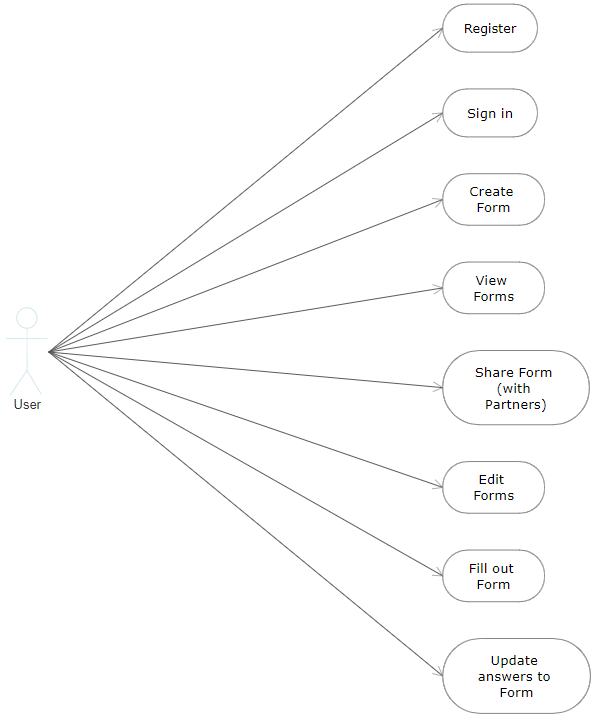
\includegraphics[height=100mm, width=150mm]{../figures/UseCaseUser}
        \caption{Use Case Diagram 1}
    \end{figure}

    \begin{figure}[h]
        \center
        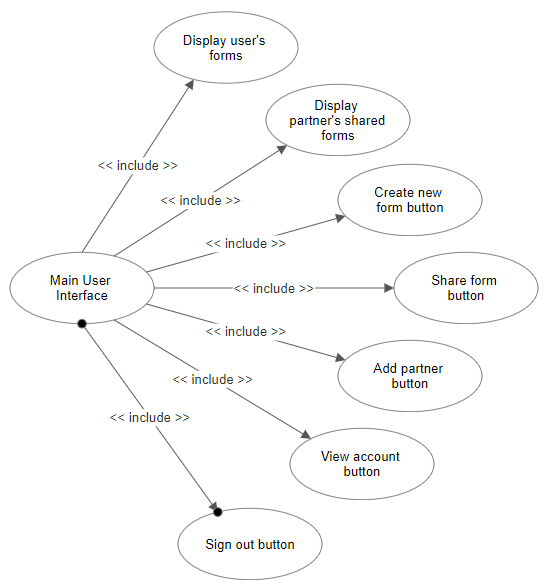
\includegraphics[width=150mm]{../figures/UseCaseInterface}
        \caption{Use Case Diagram 2}
    \end{figure}

    \clearpage

    \subsection{Use Case Description}

        The following table explains the major use cases for the application:\\

        \begin{table}[h]
            \centering
            \begin{tabular}{|c|c|}
                \hline
                Use Case & Description\\
                \hline
                \hline
                Display user's forms & \makecell{A list of forms created by the user will be displayed, with\\the form's name, owner and date of last modification.}\\
                \hline
                \makecell{Display partner's\\shared form} & \makecell{A list of forms shared with the user by a partner will be\\displayed, with the form's name, owner and date of\\last modification.}\\
                \hline
                \makecell{Create new\\form button} & Takes the user to a page where they can design a new form.\\
                \hline
                Share form button & \makecell{Allows the user to share forms they have created with partners.}\\
                \hline
                Add partner button & \makecell{Allows the user to search for other people's accounts on\\the application, and add them as partners. This should\\be done with other users that one would wish to share\\ forms with and/or receive forms from.}\\
                \hline
                View account button & \makecell{Allows the user to view their account information and edit\\it if necessary. Details such as name, email, company\\and the abilityto change the account's password.}\\
                \hline
                Sign out button & Allows the user to sign out from the application.\\
                \hline
            \end{tabular}
            \caption{Use Case Descriptions}
        \end{table}

\section{Functional Requirements}
    A functional requirement defines the intended behaviour of a component or part of a system. In the table below, the major functional requirements have been described:\\

    \begin{table}[h]
        \centering
        \begin{tabular}{|c|c|}
            \hline
            Requirement & Description\\
            \hline
            \hline
            Register & \makecell{New users will create an account before being allowed to use\\the application.}\\
            \hline
            Sign in & \makecell{Users will need to log in before they are able to\\access their account, create, share and complete forms.}\\
            \hline
            Create a form & \makecell{Users will be able to create a new form, which will be saved to\\their account.}\\
            \hline
            Share a form & \makecell{Users will be able to share a form that they have created with\\a partner.}\\
            \hline
            Add a partner & \makecell{Users will be able to view and edit their account information,\\including; name, email, company and password (not viewable).}\\
            \hline
            Sign out & Users will be able to sign out of the application.\\
            \hline
            Notifications & \makecell{Users will be notified of various changes, including their partners'\\answers to forms.}\\
            \hline
        \end{tabular}
        \caption{Functional Requirements}
    \end{table}

    \subsection{Functional Requirements Analysis}
        An importance level has been assigned to each of the functional requirements, in order to effectively plan the work to be done in order to create the minimum viable product. An additional table shows how the importance levels have been determined.\\

        \begin{table}[h]
            \centering
            \begin{tabular}{|c||c|c|c|c|c|}
                \hline
                Complexity/Time & Low & Medium & High\\
                \hline
                \hline
                Short & \cellcolor{green}0.0625 & \cellcolor{green}0.125 & \cellcolor{yellow}0.25\\
                \hline
                Medium & \cellcolor{green}0.125 & \cellcolor{yellow}0.25 & \cellcolor{red}0.5\\
                \hline
                Long & \cellcolor{yellow}0.25 & \cellcolor{red}0.5 & \cellcolor{red}0.75\\
                \hline
            \end{tabular}
            \caption{Importance Levels}
        \end{table}

        \begin{table}[h]
            \centering
            \begin{tabular}{|c|c|c|c|}
                \hline
                Requirement & Complexity & Time & Importance Level\\
                \hline
                \hline
                Register & Medium & Short & \cellcolor{green}0.125\\
                \hline
                Log in & Low & Short & \cellcolor{green}0.0625\\
                \hline
                Create a form & Medium & Medium & \cellcolor{yellow}0.25\\
                \hline
                Share a form & High & Medium & \cellcolor{red}0.5\\
                \hline
                Add a partner & Medium & Medium & \cellcolor{yellow}0.25\\
                \hline
                Sign out & Low & Low & \cellcolor{green}0.0625\\
                \hline
                Notifications & Medium & Short & \cellcolor{green}0.125\\
                \hline
            \end{tabular}
            \caption{Functional Requirements Analysis}
        \end{table}

\section{Non-Functional Requirements}
    Non-functional requirements are high-level requirements, that need to be considered during the development decisions for the entire application.\\

    \begin{table}[h]
        \centering
        \begin{tabular}{|c|c|}
            \hline
            Requirement & Description\\
            \hline
            \hline
            Internet connection & \makecell{The application will be hosted online, therefore users will require\\a connection to the internet in order to access the application.}\\
            \hline
            Confidentiality & \makecell{The application will need to keep the personal information of\\ its users safe from third parties and malicious individuals.}\\
            \hline
            Integrity & \makecell{The application must present accurate information in an\\ easy-to-understand format.}\\
            \hline
            Availability & \makecell{The application must be accessible at all times. Loss of\\ Availability could lead to users leaving the application for\\ more reliable competitors.}\\
            \hline
        \end{tabular}
        \caption{Non-Functional Requirements}
    \end{table}

\section{Risk Analysis}
    The following risk analysis has been produced, based on the requirements above and potential risks to the application as a whole. A rating system, similar to that of the importance levels for the functional requirements, has been devised for the risk level.\\

    \begin{table}[h]
        \centering
        \begin{tabular}{|c||c|c|c|c|c|}
            \hline
            Consequence/Likelihood & Negligible & Minor & Moderate & Major & Catastrophic\\
            \hline
            \hline
            Impossible & \cellcolor{green}0 & \cellcolor{green}0 & \cellcolor{green}0 & \cellcolor{green}0 & \cellcolor{green}0\\
            \hline
            Low & \cellcolor{green}0 & \cellcolor{green}0.0625 & \cellcolor{green}0.125 & \cellcolor{green}0.1875 & \cellcolor{yellow}0.25\\
            \hline
            Medium & \cellcolor{green}0 & \cellcolor{green}0.125 & \cellcolor{yellow}0.25 & \cellcolor{yellow}0.375 & \cellcolor{yellow}0.5\\
            \hline
            High & \cellcolor{green}0 & \cellcolor{green}0.1875 & \cellcolor{yellow}0.375 & \cellcolor{red}0.5625 & \cellcolor{red}0.75\\
            \hline
            Certain & \cellcolor{green}0 & \cellcolor{yellow}0.25 & \cellcolor{yellow}0.5 & \cellcolor{red}0.75 & \cellcolor{red}1\\
            \hline
        \end{tabular}
        \caption{Risk Levels}
    \end{table}

    \hfill\break

    \begin{table}[h]
        \centering
        \begin{tabular}{|c|c|c|c|c|c|}
            \hline
            Risk & Likelihood & Consequence & \makecell{Risk\\Rating} & Mitigation\\
            \hline
            \hline
            \makecell{Network\\loss} & High & Minor & \cellcolor{green}0.1875 & Frequent update of database.\\
            \hline
            \makecell{Data\\loss} & Low & Catastrophic & \cellcolor{yellow}0.25 & Redundant database.\\
            \hline
            \makecell{Security\\breach} & Medium & Catastrophic & \cellcolor{yellow}0.5 & \makecell{Follow good practice for secure\\deveopment of cloud applications.}\\
            \hline
            \makecell{Function\\error} & High & Major & \cellcolor{red}0.5625 & \makecell{Implementation of test\\framework to ensure application\\is fully functional.}\\
            \hline
            \makecell{Interface\\error} & High & Major & \cellcolor{red}0.5625 & \makecell{Implementation of test\\framework to ensure application\\is fully functional.}\\
            \hline
        \end{tabular}
        \caption{Risk Analysis}
    \end{table}

\section{Functionality}
    Below is a series of diagrams which describe the flow of some of the primary pieces of functionality in the application. They show the logic behind various aspects of the application, as well as some of the infrastructure that will be in place.

    \pagebreak

    \subsection{Activity Diagrams}
    
        \begin{figure}[!h]
            \center
            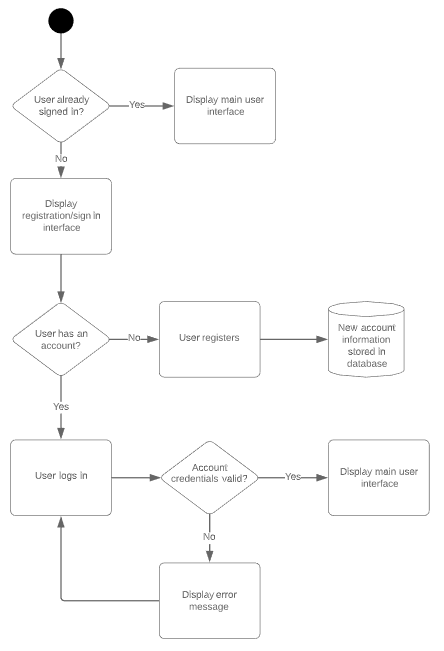
\includegraphics[width=120mm]{../figures/ActivityDiagramAuthentication}
            \caption{Activity Diagram: Authentication}
        \end{figure}

        \pagebreak

        \begin{figure}[!h]
            \center
            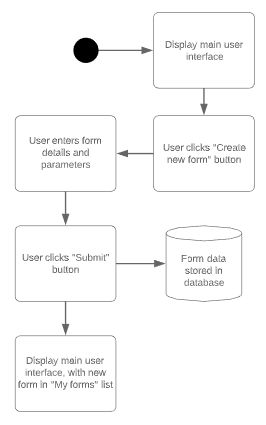
\includegraphics[width=120mm]{../figures/ActivityDiagramFormCreation}
            \caption{Activity Diagram: Form Creation}
        \end{figure}

        \pagebreak

        \begin{figure}[!h]
            \center
            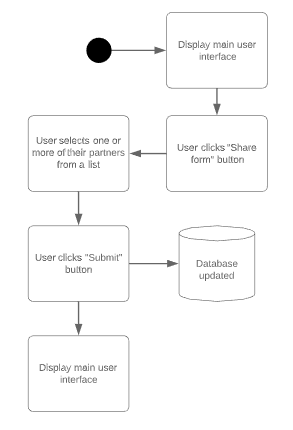
\includegraphics[width=120mm]{../figures/ActivityDiagramFormSharing}
            \caption{Activity Diagram: Form Sharing}
        \end{figure}

        \pagebreak

        \begin{figure}[!h]
            \center
            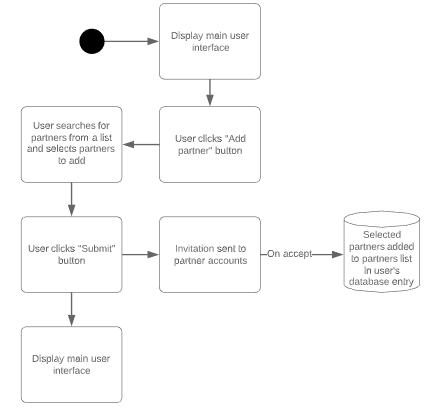
\includegraphics[width=120mm]{../figures/ActivityDiagramPartnerInvitation}
            \caption{Activity Diagram: Partner Invitation}
        \end{figure}

        \pagebreak

    \subsection{Model-View-Controller Diagram}

    \hfill\break

        \begin{figure}[!h]
            \center
            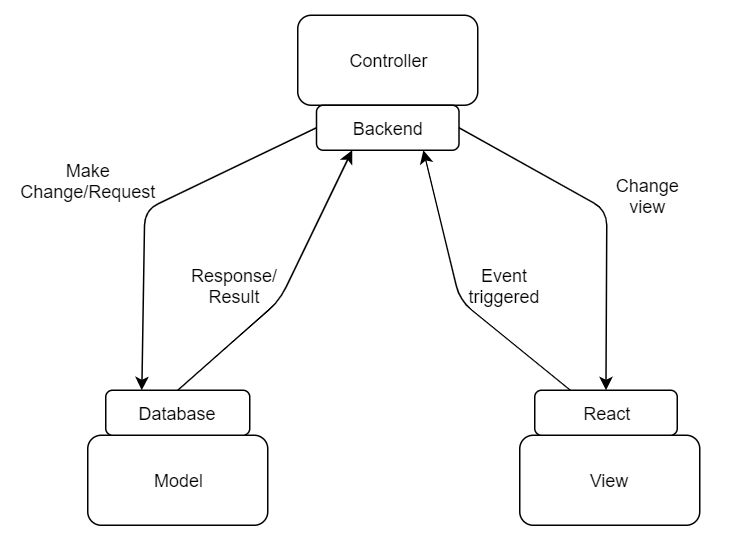
\includegraphics[width=155mm]{../figures/MVC}
            \caption{MVC Diagram}
        \end{figure}

\section{Validation}
    The testing and validation of the application will be done using Robot Framework. Robot Framework is a generic, open source, automation framework for acceptance testing \cite{Robot}, developed with Python. The framework has many libraries that extend its functionality, and one such library is Selenium, which will be used extensively to automatically drive the application\textquoteright s user interface. These tests will be written in conjunction with the application\textquoteright s features, and run alongside each check-in, as per the continuous integration methodology.
%% ----------------------------------------------------------------
%% Conclusions.tex
%% ---------------------------------------------------------------- 
\chapter{Conclusions} \label{Chapter: Conclusions}


% \backmatter means that we've gone from 1,2,3,4,5 chapter numbering 
% to unnumbered bibliography/appendices. 
\backmatter

\bibliographystyle{src/IEEEtran}
\bibliography{master}
\appendix
% %% ----------------------------------------------------------------
%% Appendix.tex
%% ---------------------------------------------------------------- 
\chapter{Appendix A: Photos} \label{appendix1}
This is an appendix

\chapter{Appendix B: Code Listings} \label{appendix2}
This is an appendix

\end{document}
